%************************************************
\chapter{Desarrollo}\label{ch:desarrollo}
%************************************************

En la primer sección de este capítulo se brindarán detalles del prototipo de dispositivo de medición mediante luz estructurada, junto con las características de sus principales componentes. 
En la segunda sección se hablará superficialmente de las principales características del software involucrado.
En la tercera sección se justificará la elección de los patrones de luz estructurada que se utilizarán y se explicará de manera simple la forma en que se usan, siendo el punto más importante su decodificación de manera robusta. 
En la cuarta sección se tratará la obtención de la nube de puntos en tres dimensiones a partir del uso de las imagenes de los patrones decodificados. 
La sección siguiente se dedicará específicamente al proceso de calibración y las herramientas desarrolladas para tal fin. 
En la última sección se analizarán las más importantes limitaciones del dispositivo.

\section{Prototipo}

\begin{figure}[!bth]
    \myfloatalign
        {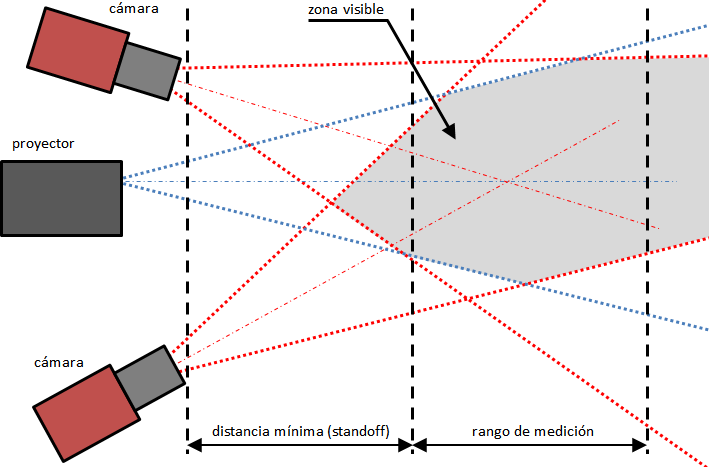
\includegraphics[width=1.0\linewidth]{images/setup/setupSchema}}
%        {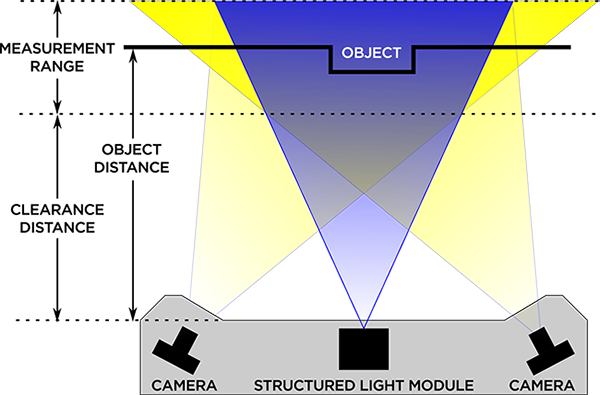
\includegraphics[width=1.0\linewidth]{images/lmi3d/Gocator-3100-howitworks}}
        \caption{Esquema del prototipo}
        \label{fig:prototypeDiagram}
\end{figure}

El prototipo desarrollado cuenta con dos cámaras y un proyector, dispuestos como se indica en la \autoref{fig:prototypeDiagram}.
Se puede observar que existe una zona con límites bien definidos, que denominaremos zona visible, que corresponde a la intersección del campo de visión de las cámaras junto con el campo de proyeccion del proyector. También se observa una distancia mínima y un rango de medición. Estos límites son difusos (a diferencia de la zona visible) y se establecen debido a que las lentes (tanto de las cámaras como del proyector) tienen una profundidad de foco acotada. La calibración se ajusta para realizar mediciones dentro de este rango. Por más que sea posible obtener mediciones en cualquier parte de la zona visible, no se puede brindar ninguna garantía respecto a la cota de error en las mediciones obtenidas fuera del rango de medición.

El esquema propuesto es el utilizado en sensores comerciales como los que ofrece Geomagic (ahora parte de 3D Systems) con su producto Geomagic Capture\footnote{\url{http://geomagic.com/en/products/capture/overview/}}, LMI3D con su producto Gocator Snapshot Sensor\footnote{\url{http://lmi3d.com/products/gocator/snapshot-sensor/}}, GOM a traves de sus diversos escaners 3D\footnote{\url{http://www.gom.com/metrology-systems/3d-scanner.html}}, entre otros (ver \autoref{fig:dispositivosComerciales}).
La mayoría de estos productos vienen calibrados de fábrica y no permiten al usuario realizar modificaciones para adaptarlos a requerimientos particulares. El prototipo armado está compuesto por piezas de laboratorio que permiten gran flexibilidad para realizar ajustes y modificaciones, y se desarrolló un procedimiento relativamente sencillo para facilitar su calibración.

\begin{figure}[!bth]
    \myfloatalign
        \subfloat[Geomagic Capture]{
            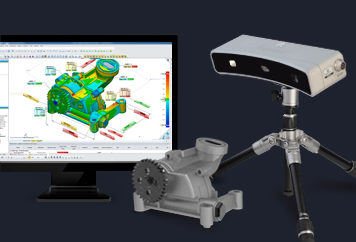
\includegraphics[width=0.58\linewidth]{images/geomagic/inspection_page_graphic_v2}
        }
        \subfloat[Gocator Snapshot Sensor]{
            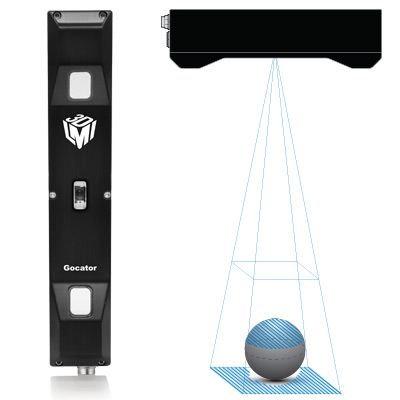
\includegraphics[width=0.40\linewidth]{images/lmi3d/snapshot-sensor-banner}
        }
        \\
        %\subfloat{
        %    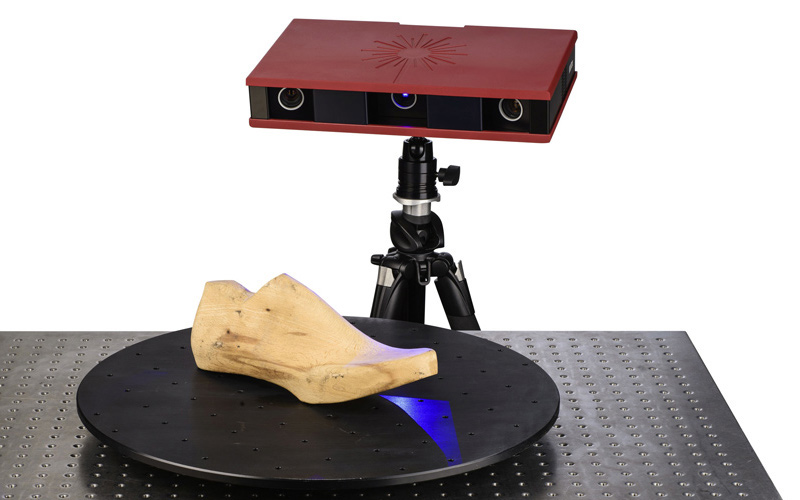
\includegraphics[width=0.49\linewidth]{images/gom/atos-core_03}
        %}
        \subfloat[GOM ATOS 3D Scanner]{
            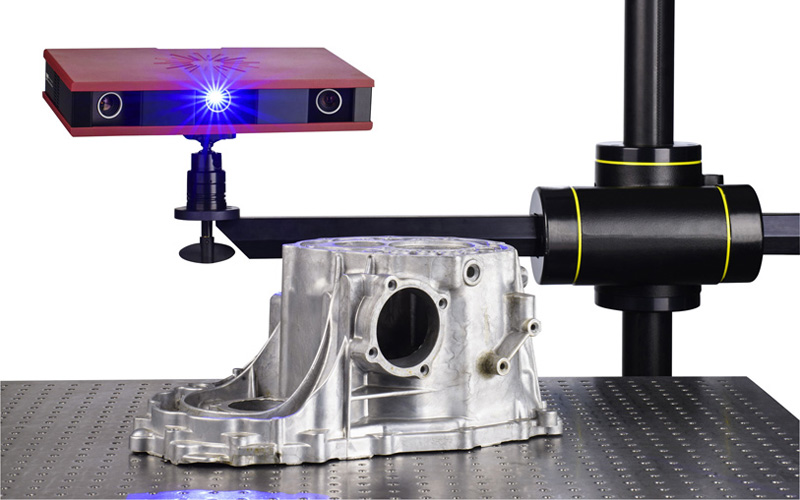
\includegraphics[width=0.49\linewidth]{images/gom/atos-core_04}
            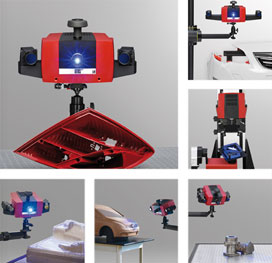
\includegraphics[width=0.49\linewidth]{images/gom/atos-compact-scan_01}
        }
        \caption{Dispositivos comerciales}
        \label{fig:dispositivosComerciales}
\end{figure}



\subsection{Componentes}
Los principales componentes del prototipo son:

\begin{itemize}
%    \item cámara Point Grey Chameleon CMLN-13S2M-CS\footnote{\url{http://ww2.ptgrey.com/USB2/chameleon}}
%    \item cámara Lumenera LM165M\footnote{\url{http://www.lumenera.com/products/industrial-cameras/lm165.php}}
    \item cámara Allied Vision Technologies Prosilica $GE1910$\footnote{\url{http://www.alliedvisiontec.com/us/products/cameras/gigabit-ethernet/prosilica-ge/ge1910.html}}
    \item cámara Allied Vision Technologies Prosilica $GC2450$\footnote{\url{http://www.alliedvisiontec.com/us/products/cameras/gigabit-ethernet/prosilica-gc/gc2450.html}}
    \item $2$ lentes de $16$ mm de distancia focal
    \item proyector Texas Instruments DLP Pico Projector Development Kit\footnote{\url{http://www.ti.com/tool/dlp1picokit}}
\end{itemize}

Se elige la utilización de cámaras en escala de grises (no color) ya que estas son más eficientes respecto a la adquisición de la luz y tienen menor ruido\footnote{Esto se debe en gran medida a que las cámaras monocromáticas no incorporan lo que se conoce como filtro de bayer (ver \url{http://en.wikipedia.org/wiki/Bayer_filter}), el cual es necesario para obtener imágenes color. Existen otros métodos para obtener imágenes color pero éste es el más utilizado.}. Las cámaras brindan la posibilidad de ser controladas por una señal de \emph{trigger} (por hardware), sin embargo para las pruebas no se las utiliza de esta manera sino que son controladas y sincronizadas completamente por software.

El proyector es de bajo consumo y reducidas dimensiones, pero también de baja resolución: solamente $480x320$ pixeles. La ventaja de este proyector está en la utilización de tecnología DLP de Texas Instruments. Se trata básicamente de un proyector que genera la imagen a partir de una fuente de luz LED y una grilla de espejos en miniatura. El diagrama del funcionamiento de un espejo puede verse en la \autoref{fig:dlpMirrorOpticalDiagram}. Este tipo de tecnología posibilita generar patrones binarios con frecuencias mayores a 2KHz. Si bien en el prototipo no estamos utilizando esta ventaja (ya que se lo utiliza de igual manera que un proyector común de computadora), se debe tener en cuenta que el dispositivo brinda esta posibilidad, pudiendo ser aprovechada a futuro mediante el uso de cámaras de alta velocidad y sincronización por hardware.

\begin{figure}[!bth]
    \myfloatalign
%        {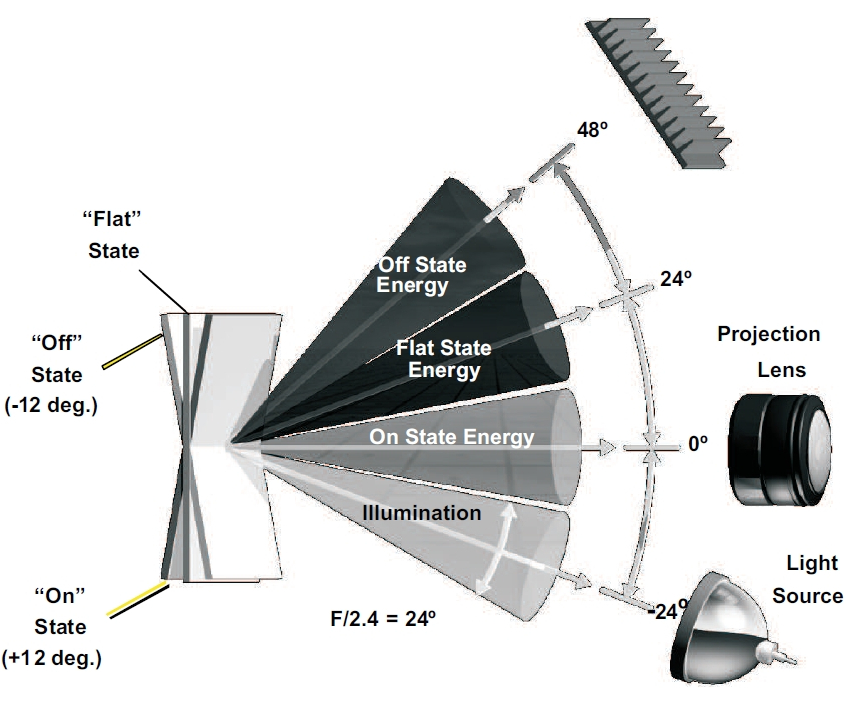
\includegraphics[width=1.0\linewidth]{images/DLP_mirrorOpticalDiagram}}
        {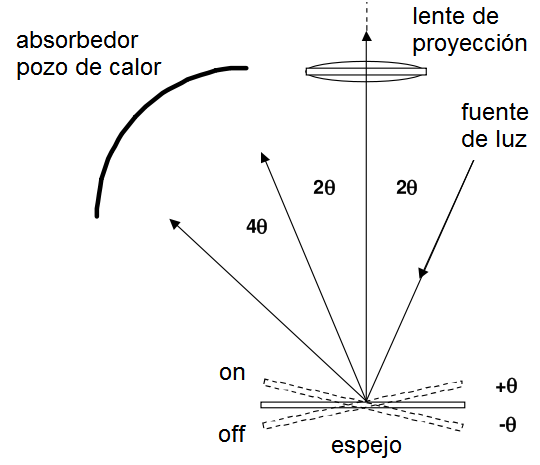
\includegraphics[width=0.7\linewidth]{images/schema-dlp}}
        \caption{Diagrama de funcionamiento de la tecnología DLP}
        \label{fig:dlpMirrorOpticalDiagram}
\end{figure}


\section{Software}
El software se implementó en lenguaje C++ utilizando el framework open-source multiplataforma Qt\footnote{\url{http://qt-project.org/}} y la biblioteca OpenCV\footnote{\url{http://opencv.org/}}. El principal objetivo del software es facilitar el uso del dispositivo (fundamental en el caso de un usuario inexperto) y ayudar al desarrollador a implementar nuevos tipos de patrones de luz estructurada y visualizar resultados para depurar los algoritmos. 
Para lograr una buena interacción con el usuario se brinda una interfaz de usuario simple que permite el acceso a la mayoría de las opciones, pero evitando sobrecargarla demasiado con todos los parámetros internos.
En el caso del desarrollador (tanto actual como los posibles futuros interesados en contribuir), se diseñó una estructura completamente modular, con diferentes bibliotecas dedicadas exclusivamente a las principales funcionalidades: adquisición de imágenes, calibración de la cámara, sistemas de luz estructurada, visualización de nubes de puntos en 3D, etc.

Una de las características más destacadas es la implementación de una biblioteca genérica para la adquisición de imágenes de distintas marcas y modelos de cámaras, la cual utiliza plugins para incorporar la funcionalidad de cada \ac{SDK} utilizado. El uso de plugins permite incorporar facilmente nuevos modelos y marcas de cámaras o \ac{SDK} mediante el uso de una \ac{API} bien definida y con la ventaja de que no requiere la recompilación del software que los utiliza. Por otro lado también permite reducir considerablemente las dependencias en tiempo de ejecución, favoreciendo la utilización (o no) de ciertos plugins en base a los requerimientos de las cámaras utilizadas. Actualmente se pueden utilizar las cámaras de Point Grey soportadas por su FlyCapture SDK\footnote{\url{http://www.ptgrey.com/flycapture-sdk}}, las cámaras de Lumenera soportadas por su LuCam SDK\footnote{\url{http://www.lumenera.com/support/downloads/industrial-downloads.php}}, las cámaras de Allied Vision Technologies soportadas por su Vimba SDK\footnote{\url{http://www.alliedvisiontec.com/us/products/software/vimba-sdk.html}}, todas las cámaras GigE, 10 GigE, USB 2.0, USB 3.0 y WIFI soportadas por el eBUS SDK de Pleora\footnote{\url{http://www.pleora.com/our-products/ebus-sdk}} y todas las cámaras soportadas por NI-IMAQdx de National Instruments\footnote{\url{http://sine.ni.com/nips/cds/view/p/lang/es/nid/207702}}.

En la \autoref{fig:scannerSoft_mainWindow} se puede observar la ventana principal de la aplicación y la configuración de una cámara. El menú superior de la ventana principal contiene menúes para el acceso a la configuración, vista previa y calibración de las cámaras; como así también acceso a la ventana para visualizar en tres dimensiones la ubicación física de las cámaras ó el resultado de la medición en el sistema de coordenadas global.

\begin{figure}[!bth]
    \myfloatalign
        \subfloat[Ventana principal]{
            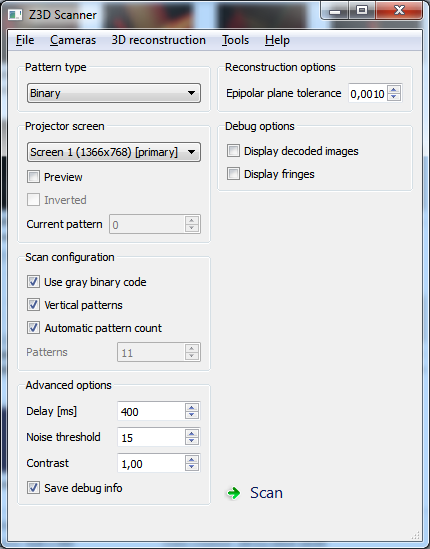
\includegraphics[width=0.49\linewidth]{images/soft/scannerSoft_mainWindow_win7}
        }
        \subfloat[Opciones de la cámara]{
            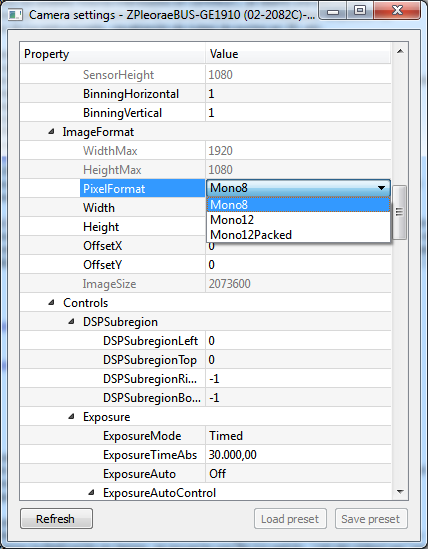
\includegraphics[width=0.49\linewidth]{images/soft/scannerSoft_cameraSettings_win7}
        }
        \caption{Software de medición}
        \label{fig:scannerSoft_mainWindow}
\end{figure}


\section{Proyección y decodificación de los patrones}
Para la codificación y decodificación se parte de la suposición de que la escena es estática (o se puede considerar estática durante el período de escaneado), ya que utilizamos una codificación temporal. Se proyectan multiples patrones y la secuencia temporal de valores para cada pixel se utiliza como código.

La codificación que utilizaremos se basa en patrones binarios debido a que es más robusta al ruido. En la parte superior de la \autoref{fig:grayCodeExample} se puede observar un ejemplo de la codificación en binario Gray (se muestran como blanco y negro los dos valores posibles, 0 y 1). Como realizamos multiplexación en tiempo, se proyecta una fila (un patrón, 1 bit del código) por vez. Utilizamos patrones con franjas verticales, por lo que el valor de una fila se repite para toda la columna, como se puede ver en la parte inferior de la \autoref{fig:grayCodeExample}. Se utiliza código Gray por sus ventajas ya mencionadas en la \autoref{sec:structuredLightBinary1DPatterns}.

\begin{figure}[bth]
        \myfloatalign
        \subfloat[Código gray de 8 bits. Cada fila representa un bit (un patrón de luz estructurada) y cada columna es un código único]
        {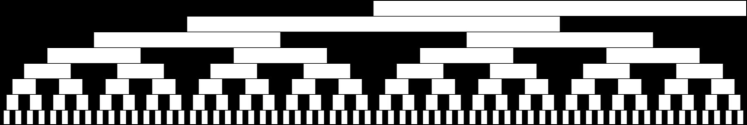
\includegraphics[width=1.0\linewidth]{images/grayCodeExample}} 
        \\
        \subfloat[Primeros 4 patrones proyectados, correspondientes a las primeras 4 filas]
        {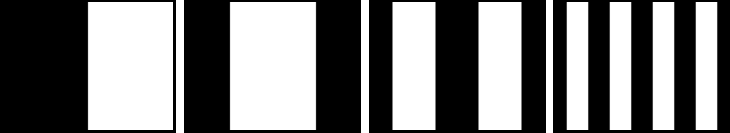
\includegraphics[width=1.0\linewidth]{images/grayCodeProjectionExample}}
        \caption{Patrones de luz estructurada usando código gray}
        \label{fig:grayCodeExample}
\end{figure}

%La elección de utilizar patrones binarios se debe principalmente a que este tipo de patrones brinda una codificación única para cada pixel, lo que hace que su decodificación sea muy robusta, y por otro lado también es relativamente simple de implementar. El uso de un patrón del tipo \emph{phase shift} puede brindarnos una mejor resolución lateral, y se podría aprovechar la ventaja que nos brinda el conocer que los objetos que se desean medir tienen superficies suaves y geometrías simples. Sin embargo el hecho de que no podemos permitirnos ambiguedades en la decodificación nos obligaría a incluir al menos un patrón de algún otro tipo que permita establecer un punto de referencia, ya que se debe conocer la fase absoluta en al menos un punto a partir del cual continuar la decodificación de la fase absoluta para todos los pixels. Por otro lado la resolución espacial que se logra resulta suficiente, ya que no es un factor crítico la detección de características puntuales. 

Para facilitar la detección de las zonas donde el patrón está presente y es visible por la cámara, y para determinar un umbral mínimo de la \emph{calidad} del pixel, se utiliza un patrón extra que es completamente blanco, y su inverso completamente negro. Este patrón se utiliza como \emph{máscara} para procesar solamente los pixels que contienen información útil.

Por otro lado, para hacer aún más robusta la decodificación y poder discernir claramente cual es el valor binario correspondiente a cada pixel, se utiliza el patrón en conjunto con su patrón inverso, como se propone en \cite{trobina1995error}. De esta forma la clasificación del valor binario correspondiente se lleva a cabo mediante la comparación de si el valor del pixel es mayor para la imagen del patrón o para la imagen del patrón inverso. Un ejemplo de la proyección de un patrón y el patrón inverso correspondiente puede observarse en la \autoref{fig:ejemploProyeccionPatronInverso}.

\begin{figure}[!bth]
    \myfloatalign
        \subfloat[Patrón]{
            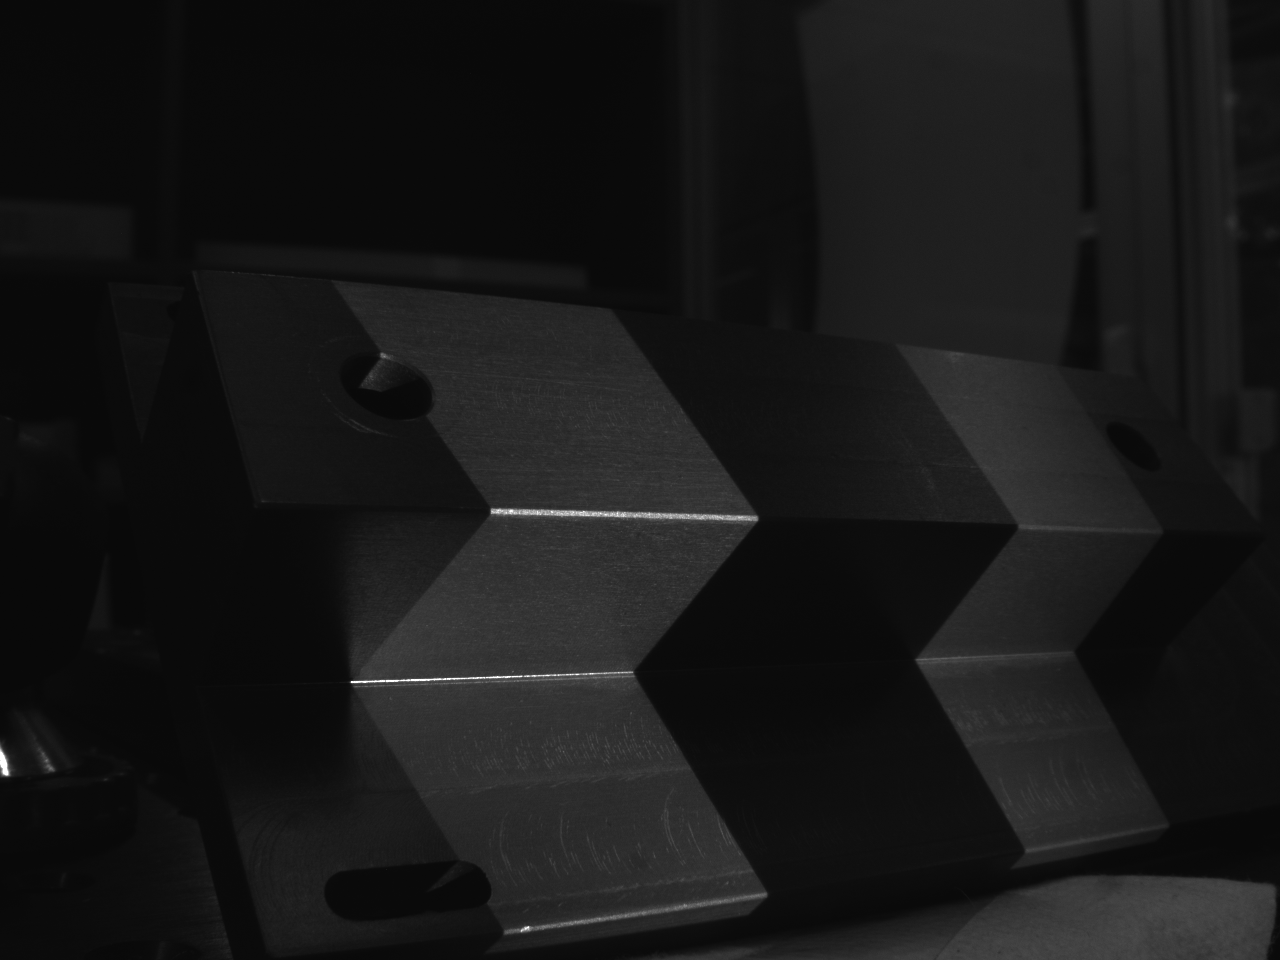
\includegraphics[width=0.49\linewidth]{images/snapshots_scan/SIMULATED-LEFT-LUMENERA-SN8010129/gray_07}
        }
        \subfloat[Patrón inverso]{
            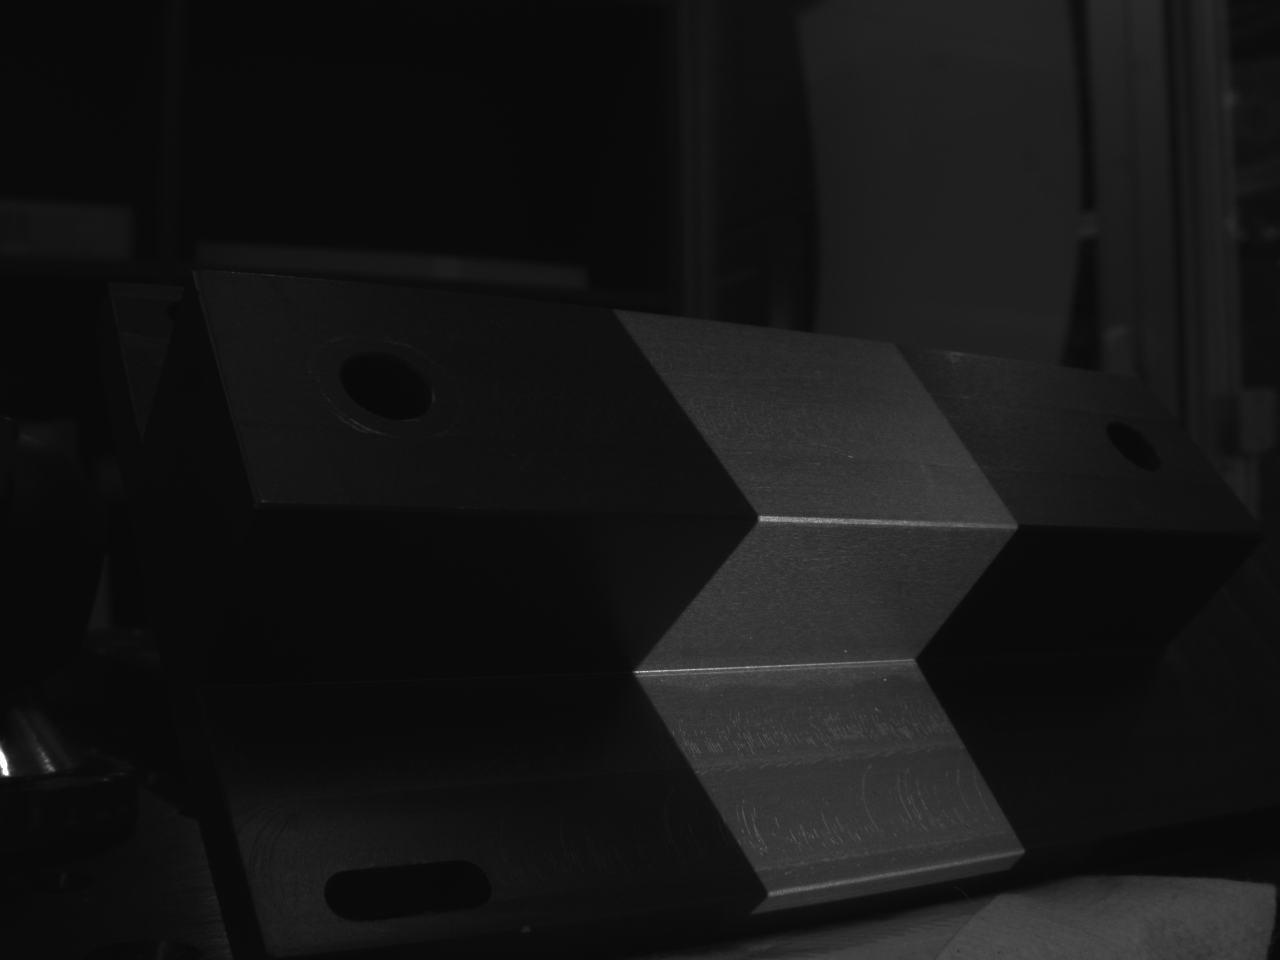
\includegraphics[width=0.49\linewidth]{images/snapshots_scan/SIMULATED-LEFT-LUMENERA-SN8010129/gray_07_inv}
        }
        \caption{Ejemplo de la proyección de un patrón y el patron inverso correspondiente}
        \label{fig:ejemploProyeccionPatronInverso}
\end{figure}

Para la obtención de las imágenes de los patrones se considera que las cámaras y el proyector están bien configurados (todos los parámetros, incluyendo tanto la configuración del sensor de la cámara como los ajustes manuales de apertura y foco del lente). No entraremos en detalle en estas cuestiones pero la calidad de las imagenes (enfoque, nivel de ruido, contraste, etc) juega un papel fundamental en la calidad de los resultados.
Un ejemplo de un patrón observado desde ambas cámaras puede verse en la \autoref{fig:ejemploProyeccion}. En la \autoref{fig:ejemploDecodificacion} se puede observar el resultado de la decodificación para estas imágenes de ejemplo.

\begin{figure}[!bth]
    \myfloatalign
        \subfloat[Cámara izquierda]{
            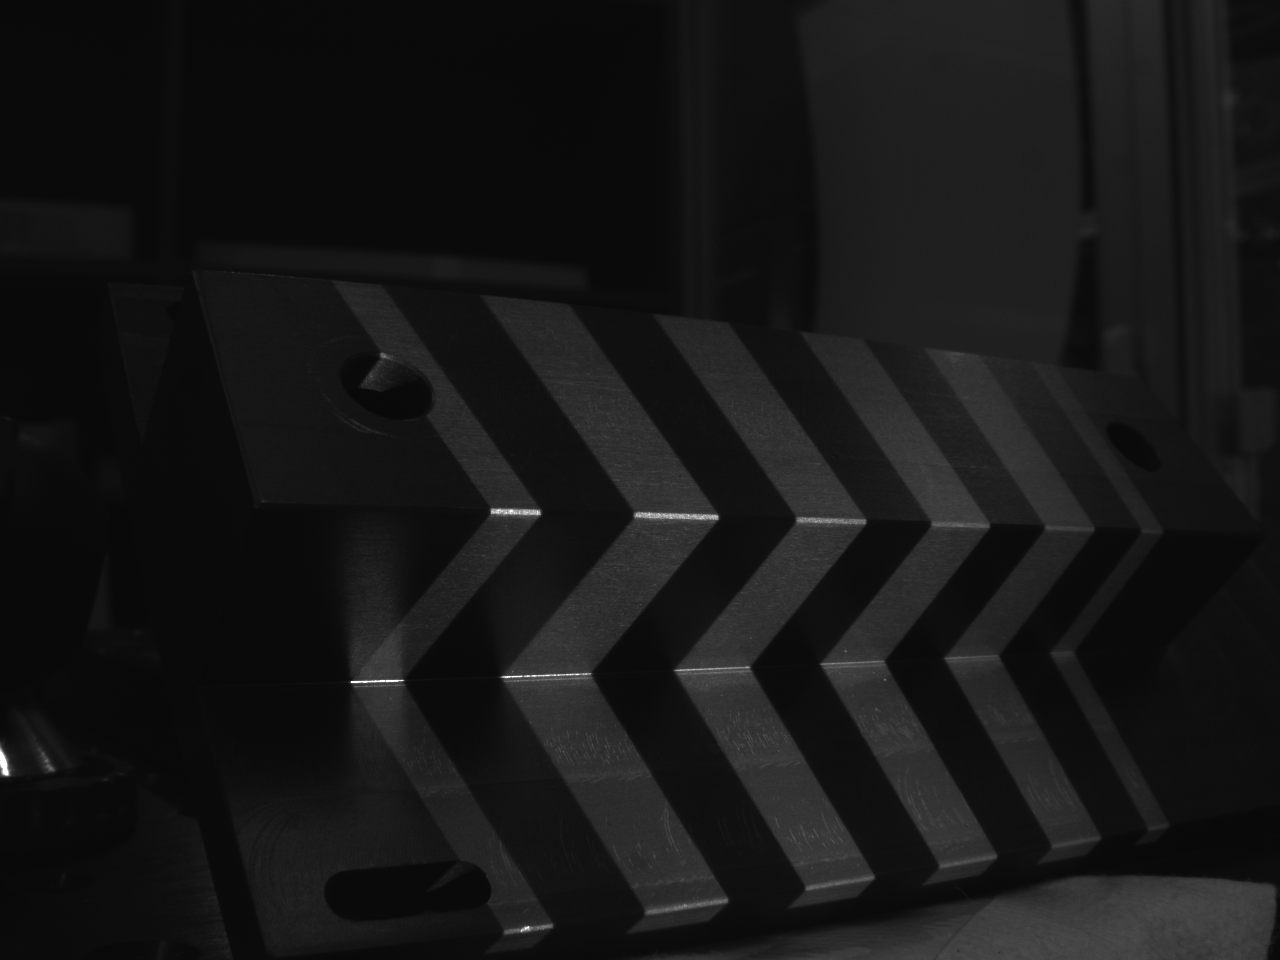
\includegraphics[width=0.49\linewidth]{images/snapshots_scan/SIMULATED-LEFT-LUMENERA-SN8010129/gray_05}
        }
        \subfloat[Cámara derecha]{
            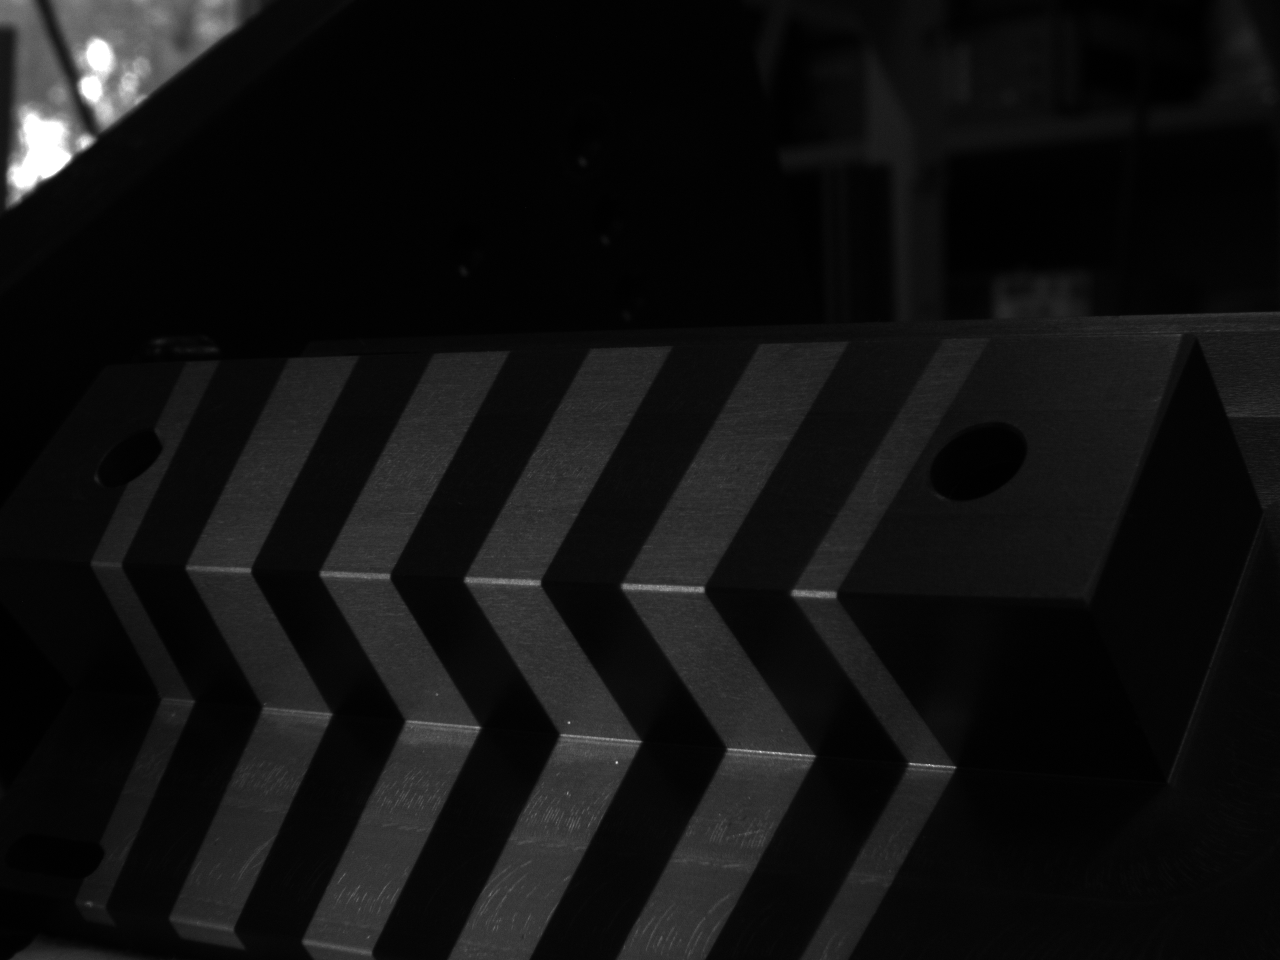
\includegraphics[width=0.49\linewidth]{images/snapshots_scan/SIMULATED-RIGHT-PGR-SN9041369/gray_05}
        }
        \caption{Ejemplo de un patrón proyectado}
        \label{fig:ejemploProyeccion}
\end{figure}

\begin{figure}[!bth]
    \myfloatalign
        \subfloat[Cámara izquierda]{
            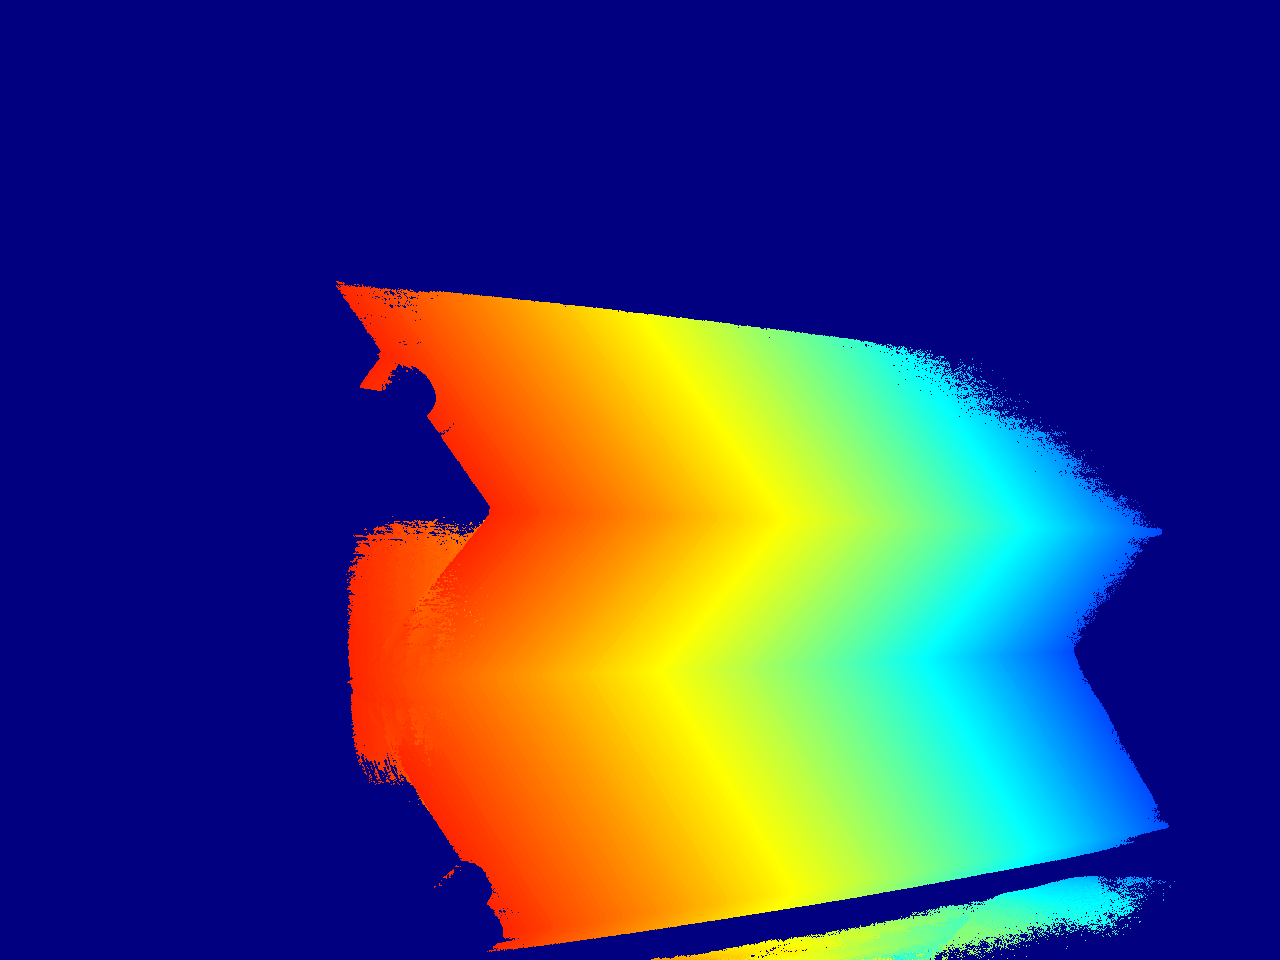
\includegraphics[width=0.49\linewidth]{images/soft/decodedLeft}
        }
        \subfloat[Cámara derecha]{
            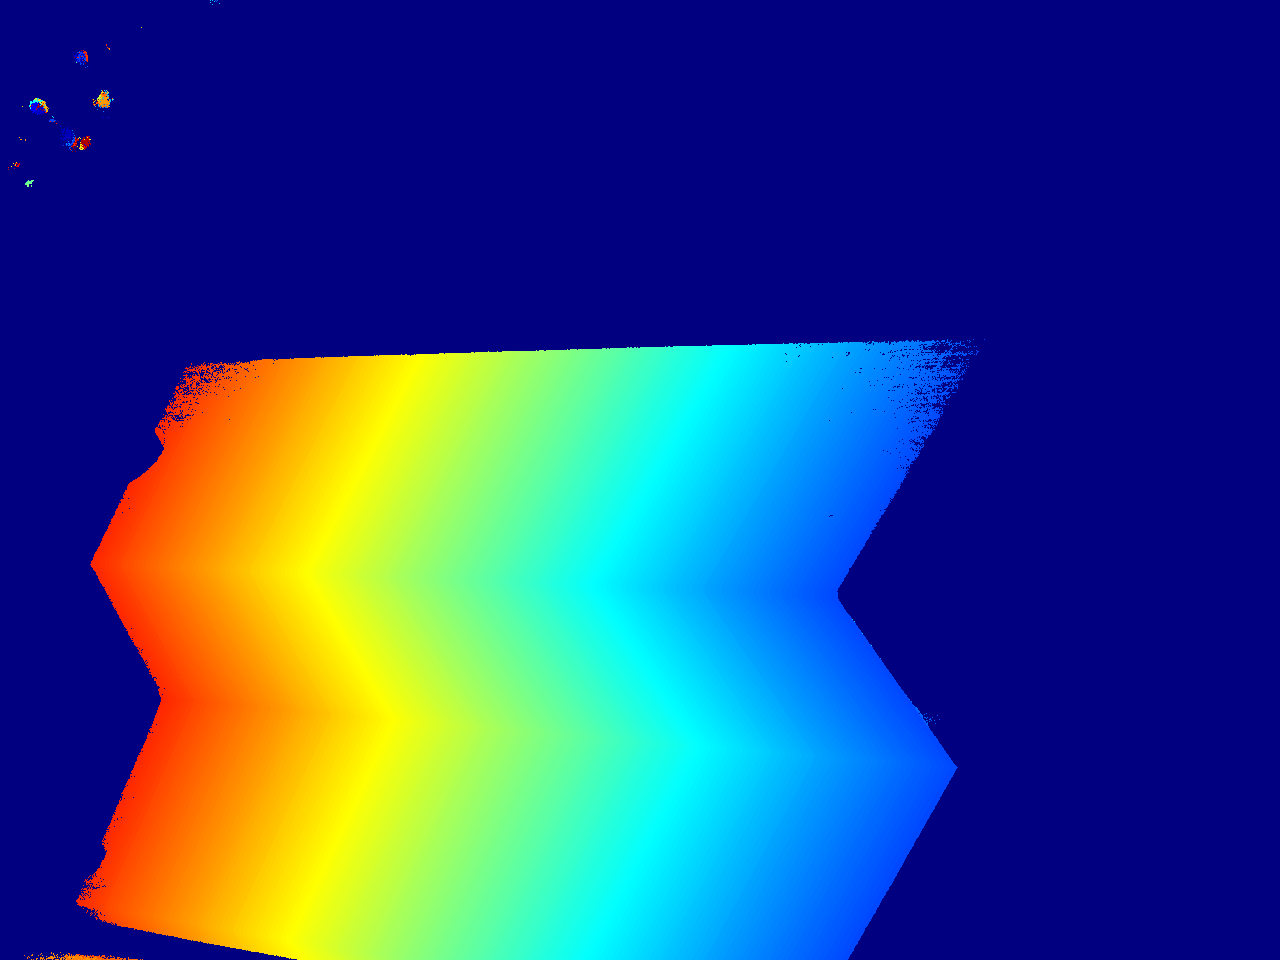
\includegraphics[width=0.49\linewidth]{images/soft/decodedRight}
        }
        \caption{Resultado de la decodificación de las imagenes. El color representa el código: en este caso el código es el valor de la columna del proyector}
        \label{fig:ejemploDecodificacion}
\end{figure}

Al usar patrones binarios, la única información útil es la representada por el límite entre una franja y la siguiente. Es decir, el valor del código de cualquier pixel dentro de una franja de pixeles con el mismo código no nos brinda información relevante\footnote{Nos sirve para conocer que ese pixel no es un hueco, que corresponde a una parte de la pieza, pero no contiene información relevante para conocer con exactitud su ubicación en el espacio}. Es por esto que lo primero que necesitamos es obtener la ubicación de los \emph{bordes} entre las franjas. Los bordes que más nos interesan son aquellos que se encuentran entre dos franjas consecutivas (con código sucesivo). En la \autoref{fig:ejemploDecodificacionBordes} se muestra el resultado de este primer procesamiento de las imagenes decodificadas, donde se eliminan todos los pixels interiores a cada franja y sólo se mantienen los bordes.

A partir de este procesamiento se generan listas de pixeles correspondientes a los límites entre franjas sucesivas. Por ejemplo se genera una lista de los pixels correspondientes al límite entre las franjas con código 1 y 2, otra lista para los pixels correspondientes al límite entre las franjas con código 2 y 3, y así sucesivamente. Esto se realiza para las imagenes decodificadas de cada cámara utilizada. Cada lista tiene un identificador para saber a qué borde pertenece, para mas adelante poder establecer las correspondencias entre las distintas cámaras (o respecto a la franja del proyector, en el caso que solamente contemos con una cámara).

En este punto podemos establecer una analogía con un escaner de línea: se puede decir que cada lista de pixels es el equivalente a una línea decodificada en un escáner de línea. De esta manera se hace evidente una de las ventajas de los métodos de luz estructuradas: con el uso de patrones binarios de 9 bits (en nuestro caso, $9 x 2 + 2 = 20$ imagenes) se puede obtener el equivalente a $2^{9} - 1 = 511$ (descartando los límites exteriores de las franjas de los extremos) o $2^{9} + 1 = 513$ (utilizando los límites exteriores de las franjas de los extremos) perfiles de un escaner de línea (donde se necesita una imagen para cada perfil).

\begin{figure}[!bth]
    \myfloatalign
        \subfloat[Cámara izquierda]{
            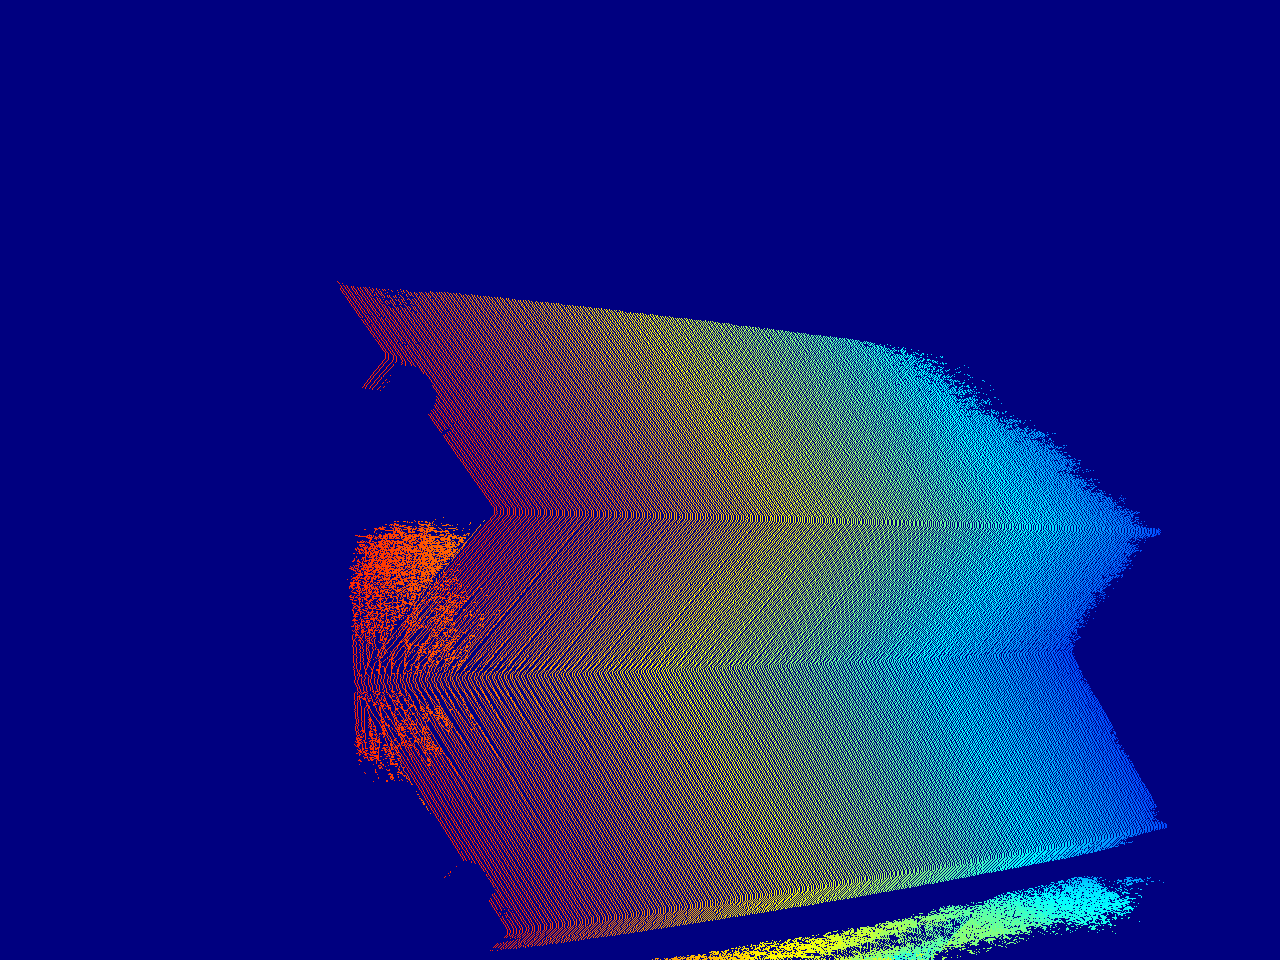
\includegraphics[width=0.49\linewidth]{images/soft/decodedBordersLeft}
        }
        \subfloat[Cámara derecha]{
            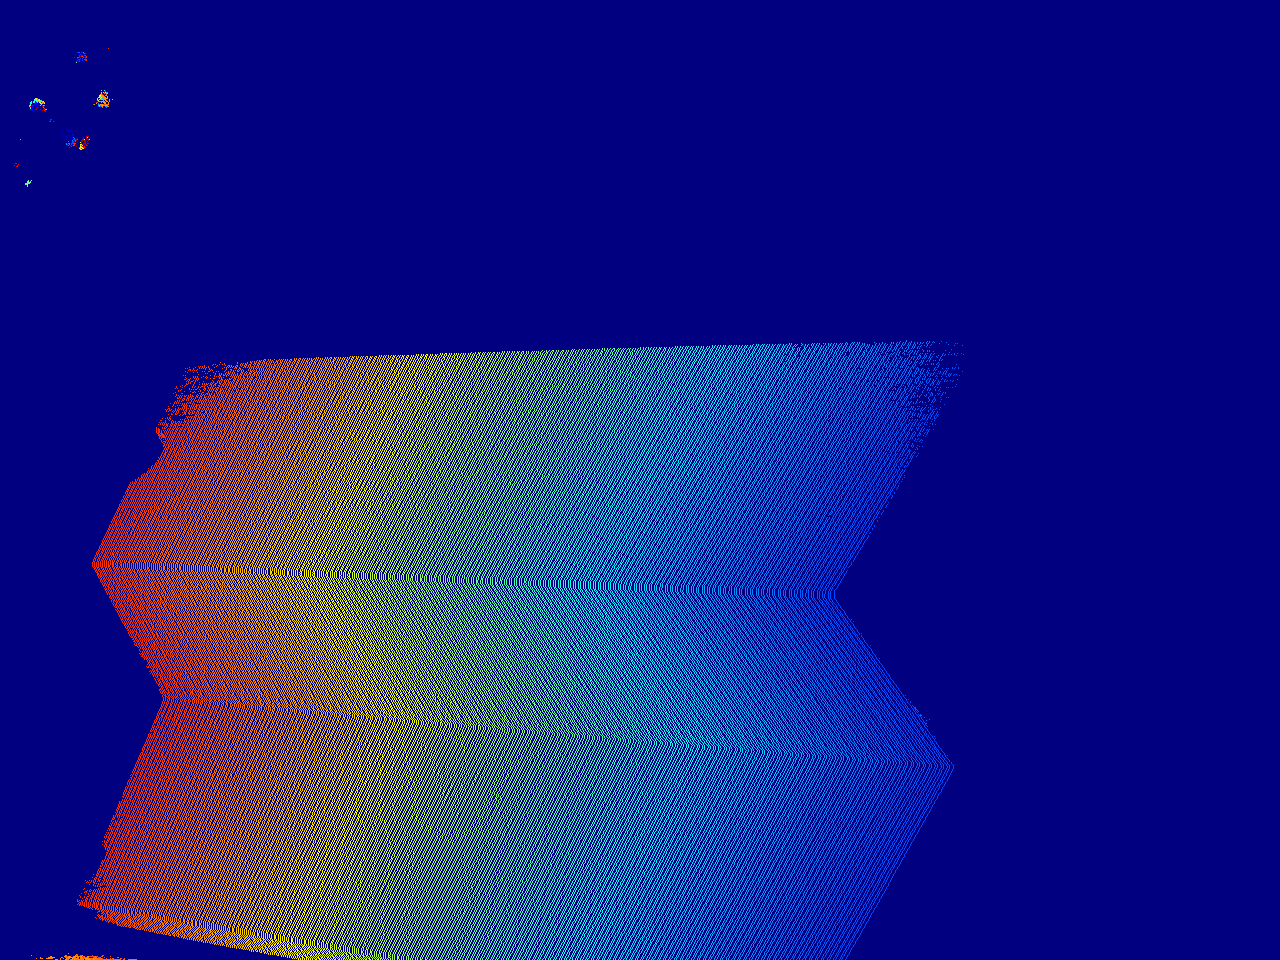
\includegraphics[width=0.49\linewidth]{images/soft/decodedBordersRight}
        }
        \caption{Bordes entre franjas decodificadas}
        \label{fig:ejemploDecodificacionBordes}
\end{figure}

En el \autoref{ch:appendixSampleScanImages} se muestra una medición de ejemplo, y se incluyen todas las imágenes que fueron utilizadas para obtenerla.

\section{Reconstrucción}

Para la obtención de la nube de puntos en tres dimensiones se deben utilizar los conceptos vistos sobre la calibración de la cámara y el principio de triangulación. En principio se asume que tenemos una buena aproximación de los parámetros del modelo de cada cámara y de su ubicación espacial respecto a un único sistema de coordenadas. Respecto al principio de triangulación utilizaremos exclusivamente la intersección entre líneas.

En esta etapa ya no utilizaremos imágenes sino el resultado de su procesamiento, es decir que partimos desde los conjuntos de coordenadas 2D de los puntos correspondientes a cada límite entre franjas. Para entender mejor el procedimiento vamos a centrarnos en el procesamiento de un solo límite entre dos franjas, es decir trataremos un sólo conjunto de puntos por cada cámara.
Conocemos que los puntos de cada conjunto corresponden a una misma línea sobre la superficie del objeto observado\footnote{Se podría decir que corresponden a un mismo plano de luz, ya que a fines prácticos podemos considerar que el proyector es perfecto. La probable deformación generada por la óptica del proyector no nos afecta.}, con lo cual mediante triangulación se puede obtener su ubicación en tres dimensiones. En este momento se puede establecer una clara relación con los conceptos involucrados en la visión estéreo, con la ventaja de que en este caso no hace falta buscar correspondencias entre las imágenes debido a que ya las conocemos por el uso patrones de luz estructurada con codificación única.

Al inicio de esta sección dijimos que ibamos a utilizar intersección entre líneas. Cada punto en la imagen (2D) puede ser transformado a una recta en el espacio (3D) mediante los conceptos ya vistos en el \autoref{ch:calibracion}. La intersección se debe realizar entre puntos de diferentes cámaras, pero todavía no establecimos la correspondencia entre los distintos puntos pertenecientes a las distintas cámaras, es decir, no conocemos qué punto del conjunto de la otra cámara debemos intersectar con cada punto de la primer cámara. 
En principio hubieramos podido reducir la complejidad de este problema agregando patrones en la dirección opuesta (en nuestro caso significaría agregar patrones con franjas horizontales), lo que nos brinda información adicional para establecer las correspondencias entre los puntos de cada conjunto. Sin embargo esto significaría la duplicación de la cantidad de patrones necesarios (y el procesamiento del doble de imágenes), con su correspondiente incremento del tiempo de medición.
Una solución práctica a este problema surge de la utilización de la geometría epipolar. Como se dijo previamente en la \autoref{sec:calibracion_intro}, el uso de un modelo de cámara central nos permite formular el mapeo como una proyección, lo que nos posibilita utilizar todos los conceptos de la geometría proyectiva \cite{hanning2011high}, incluyendo la geometría epipolar. Este concepto es muy utilizado en visión estéreo para minimizar la busqueda de correspondencias entre imágenes \cite{bradski2008learning}, y en nuestro caso nos ayuda de igual manera a reducir considerablemente el procesamiento.

La geometría epipolar nos permite realizar una proyección de las imagenes de un par de cámaras hacia un único plano de imagen virtual, el cual está a igual distancia de ambas cámaras y cuenta con el eje $x$ alineado al vector traslación que separa las dos cámaras. 
A partir de la proyección de los puntos de cada conjunto hacia este plano único podemos establecer facilmente la relación entre ellos (solamente comparamos sus coordenadas $y$ en el plano de imagen virtual) y también nos permite simplificar el cálculo de la triangulación. La intersección aproximada entre los pares de rectas (las proyecciones correspondientes a los puntos) se reduce a un cálculo muy rápido de la distancia $z$ utilizando solamente la separación en la dirección $x$ del plano de imagen virtual. Este concepto es muy utilizado en el ámbito de visión estéreo y se conoce como \emph{disparidad} (ver \autoref{fig:stereoVision}).

\begin{figure}[!bth]
    \myfloatalign
        \subfloat[Principales conceptos de la geometría epipolar]{
            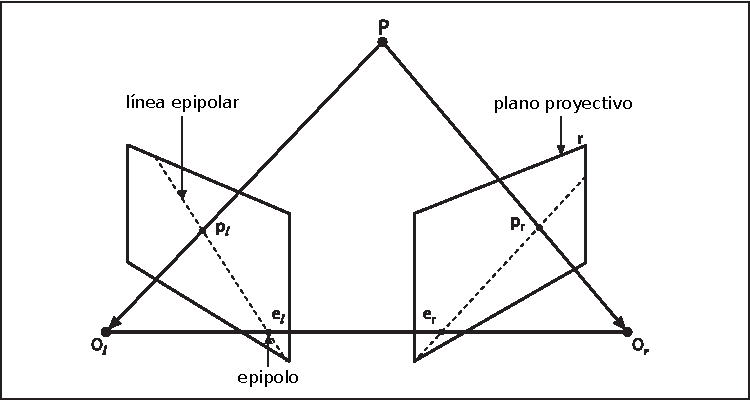
\includegraphics[width=1\linewidth]{images/epipolarPlane}
        }
        \\
        \subfloat[Proyección sobre un único plano virtual]{
            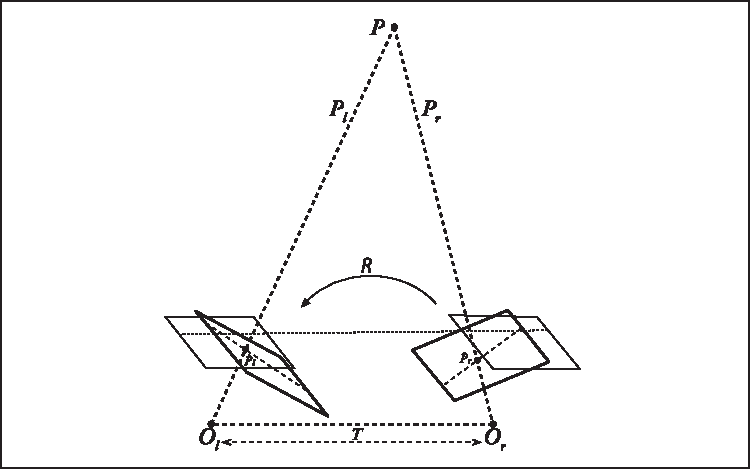
\includegraphics[width=1\linewidth]{images/epipolarPlaneCorrection}
        }
        \caption{Geometría epipolar}
        \label{fig:epipolarGeometry}
\end{figure}

Una vez que calculamos todas las intersecciones obtenemos lo que se denomina comúnmente como \emph{nube de puntos}, que no es más que un conjunto de puntos en el espacio. En este momento se puede utilizar la imágen obtenida con el patrón completamente blanco para asignarle un valor de intensidad (o color en el caso de imágenes color) a cada punto.
% (en nuestro caso no nos interesa la apariencia del objeto, pero nos permitirá visualizar el objeto de manera más realista).

Esta nube de puntos se puede utilizar como punto de partida para una gran cantidad de aplicaciones (como las mencionadas en el \autoref{ch:introduction}), y existe una gran cantidad de algoritmos y software dedicados a su procesamiento y visualización, incluyendo proyectos open-source como MeshLab\footnote{\url{http://meshlab.sourceforge.net/}} o CloudCompare\footnote{\url{http://www.danielgm.net/cc/}}, además de soluciones comerciales muy completas como SolidWorks\footnote{\url{http://www.solidworks.com/sw/products/3d-cad/scanto3d.htm}}, Geomagic Design\footnote{\url{http://geomagic.com/en/products-landing-pages/3d-design}}, SpaceClaim\footnote{\url{http://www.spaceclaim.com}}, entre muchos otros. Algunos ejemplos de las tareas que se pueden realizar son la aplicación de filtros, la reducción de la cantidad de puntos a partir de un submuestreo, la generación de superficies, la segmentación de objetos y aproximación a formas primitivas, la integración de nubes de puntos tomadas desde diferentes puntos de vista (o diversos sensores) para obtener un objeto completo, etc.
En nuestro caso lo único que nos interesa es realizar mediciones sobre formas que ya conocemos por lo que no entraremos en detalle en estos aspectos.

En la \autoref{fig:ejemploVisualizacionNubePuntos} se observa la nube de puntos obtenida para las imágenes del ejemplo. El software de visualización desarrollado es básico pero es muy útil para observar rápidamente el resultado del proceso y aplicar algunos algoritmos básicos de post-procesamiento (por ejemplo para la eliminación de valores espúreos y para realizar un suavizado de la nube de puntos). Se desarrolló con la ayuda de la biblioteca Point Cloud Libray (PCL)\footnote{\url{http://pointclouds.org/}} y del Visualization Toolkit (VTK)\footnote{\url{http://www.vtk.org/}}.

\begin{figure}[!bth]
    \myfloatalign
        \subfloat{
            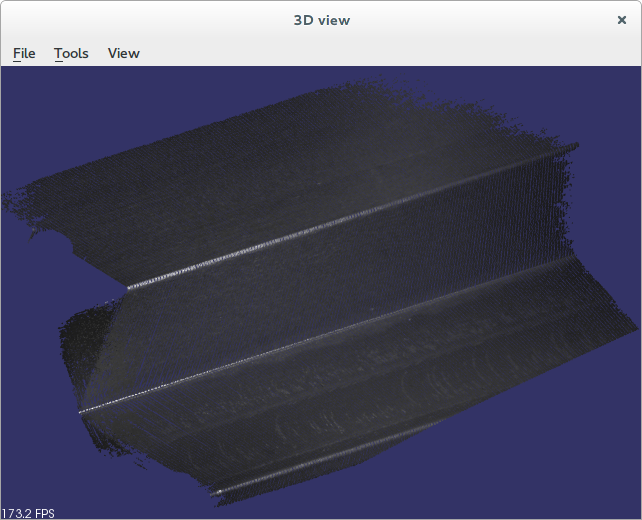
\includegraphics[width=0.8\linewidth]{images/soft/screenshot3DView}
        }
        \\
        \subfloat{
            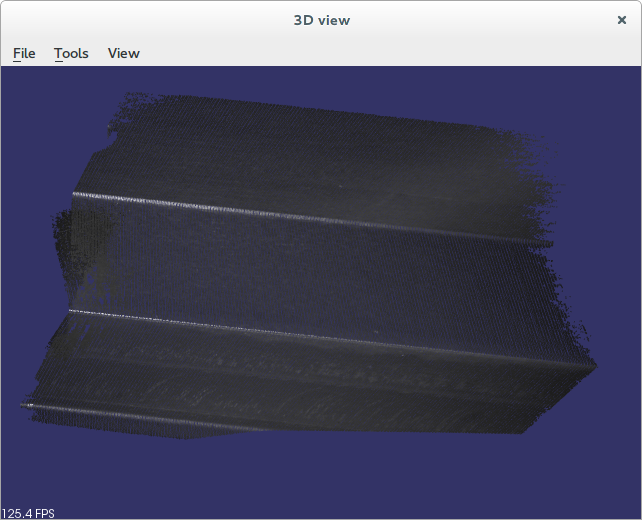
\includegraphics[width=0.8\linewidth]{images/soft/screenshot3DView2}
        }
        \\
        \subfloat{
            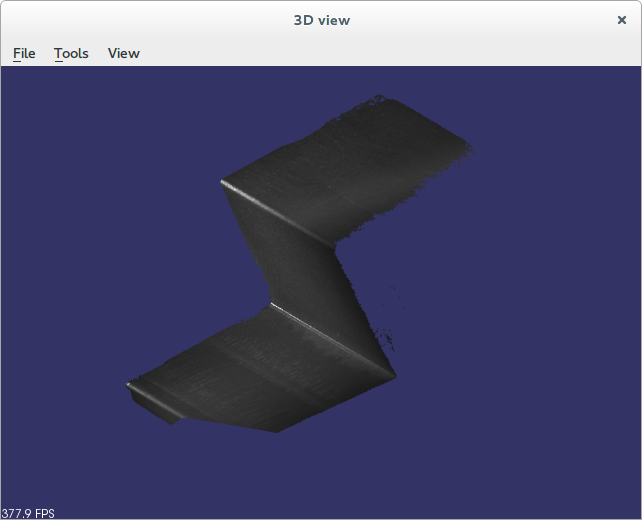
\includegraphics[width=0.8\linewidth]{images/soft/screenshot3DView3}
        }
        \caption{Visualización de la nube de puntos 3D}
        \label{fig:ejemploVisualizacionNubePuntos}
\end{figure}




\section{Calibración del dispositivo}
Junto con el software desarrollado se incluye una interfaz de usuario para facilitar la calibración de las cámaras y del dispositivo completo. En la \autoref{fig:cameraCalibrationSoft1} se observan las distintas secciones de la interfaz de calibración de los parámetros intrínsecos de las cámaras. 
Se puede ver que se incluye una sección que permite la selección del patrón de calibración a utilizar y el ajuste de los diversos parámetros del método de calibración. También cuenta con una vista previa de la cámara para tomar las fotos necesarias, permitiendo guardar las imágenes solamente cuando el patrón de calibración es detectado correctamente. El programa también incluye la funcionalidad necesaria para el uso de archivos de imágenes previamente capturadas, muy útil en caso que sea necesario repetir el procedimiento de calibración en otro momento.

Al finalizar el procedimiento de calibración se pueden guardar y actualizar los datos de la calibración actual de la cámara como así tambien observar los resultados y un mapa de colores de la magnitud de la distorsión en las distintas partes de la imagen.

Para la calibración de los parámetros intrínsecos de la cámara se recomienda utilizar sólo $4$ o $5$ imágenes del patrón de calibración en diferentes ubicaciones, pero siempre se debe tratar de que los puntos de control abarquen el mayor area posible dentro de la imagen. De esta forma aproximaremos de mejor manera la distorsión, y se evita obtener una solución que sólo aproxima bien de manera local. 

En nuestro caso, de acuerdo a la experiencia adquirida luego de varias pruebas y conociendo que el rango de medición es acotado, resulta suficiente con obtener las imagenes variando solamente la inclinación del patrón de calibración respecto a la cámara.
%La calibración es válida solamente mientras mantengamos las mismas condiciones (por ejemplo la posición del foco y apertura de la lente).
%Como el objetivo es lograr mediciones de mucha precisión, utilizamos un ángulo de triangulación relativamente alto. De esta forma la disposición de las cámaras hace que sólo sea válido cierto rango

\begin{figure}[!bth]
    \myfloatalign
        \subfloat[Parámetros de la calibración]{
            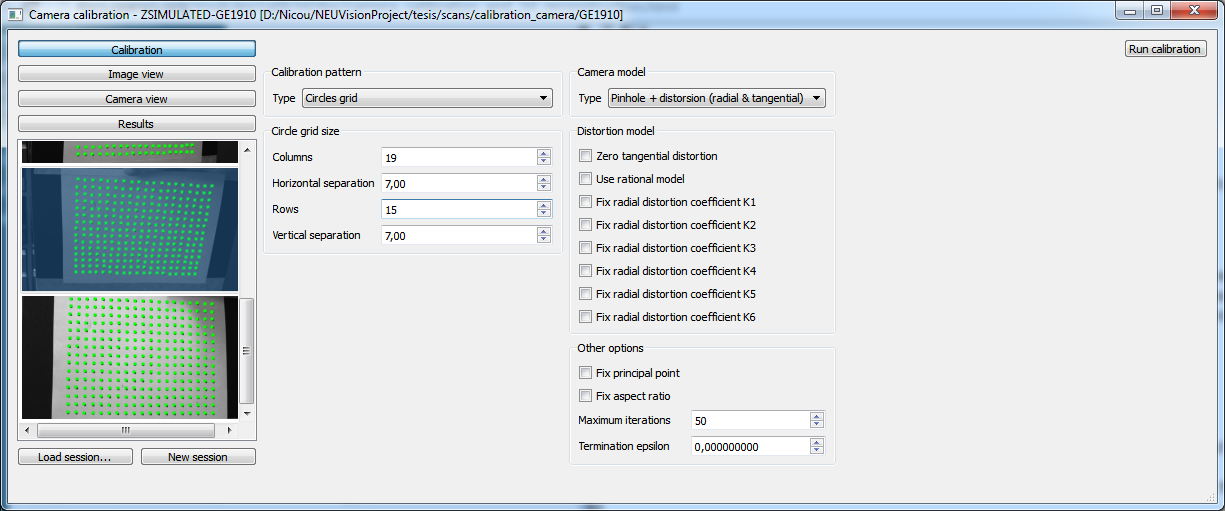
\includegraphics[width=1.0\linewidth]{images/soft/cameraCalibrationSoft_calibrationSetup_win7}
        }
        \\
        \subfloat[Vista previa de la cámara]{
            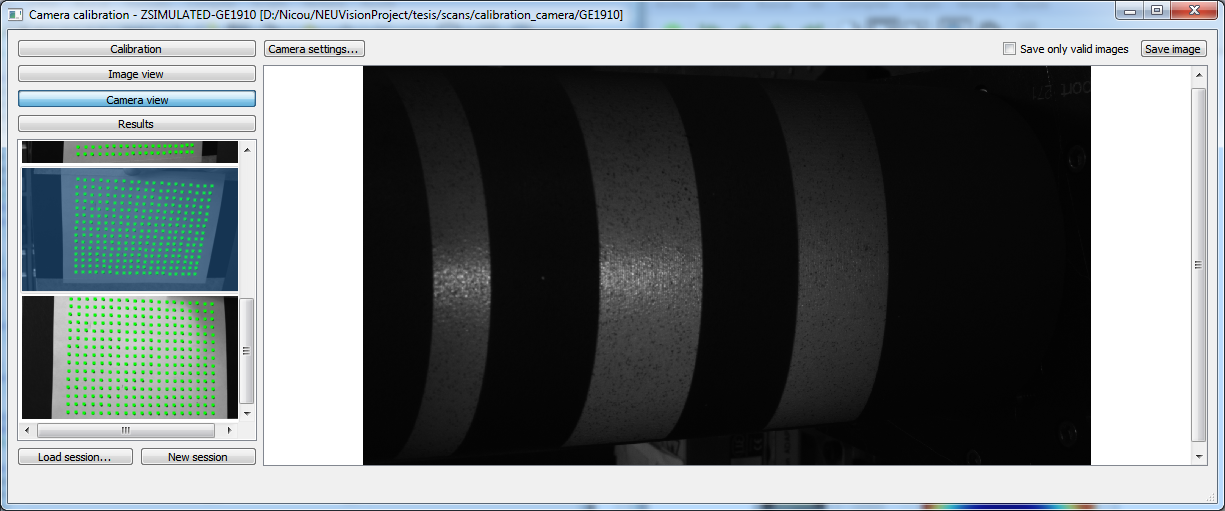
\includegraphics[width=1.0\linewidth]{images/soft/cameraCalibrationSoft_liveCameraView_win7}
        }
        \\
        \subfloat[Visor de imágenes adquiridas/guardadas]{
            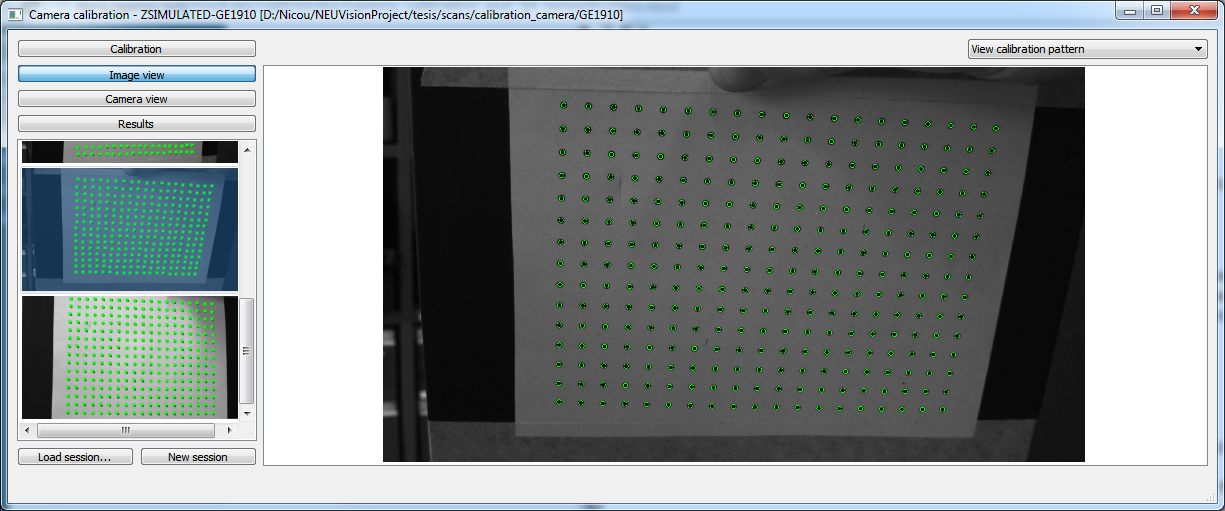
\includegraphics[width=1.0\linewidth]{images/soft/cameraCalibrationSoft_imageView_win7}
        }
        \\
        \subfloat[Resultados de la calibración]{
            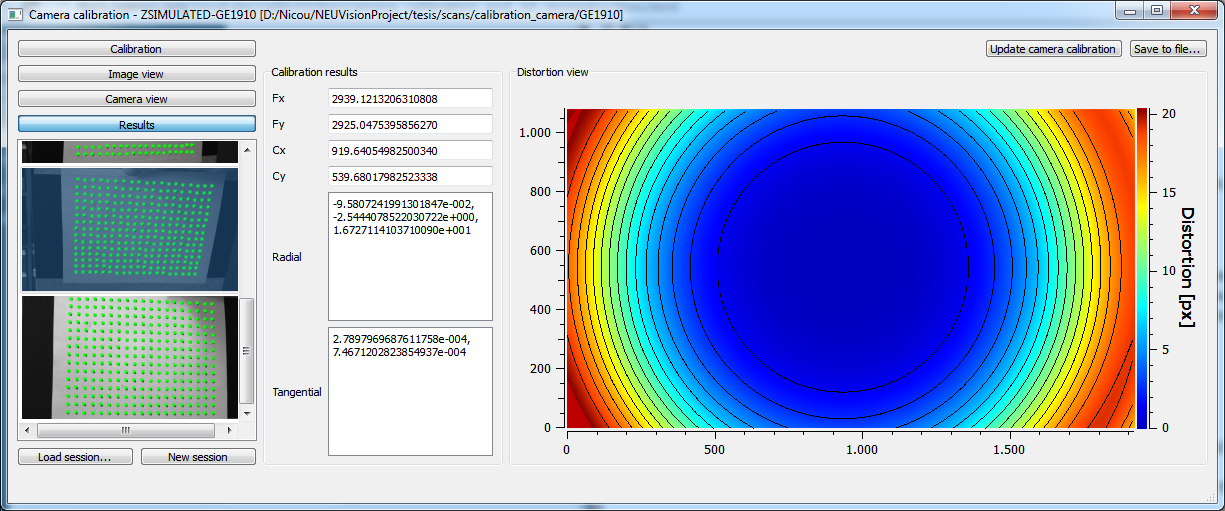
\includegraphics[width=1.0\linewidth]{images/soft/cameraCalibrationSoft_calibrationResults_win7}
        }
        \caption{Software de calibración de la cámara}
        \label{fig:cameraCalibrationSoft1}
\end{figure}

Para completar la calibración del dispositivo debemos obtener los parámetros que permiten relacionar las cámaras respecto a un único sistema de referencia. Para esto necesitaremos imágenes donde el patrón de calibración es observado simultáneamente por ambas cámaras. En este caso se recomienda el uso de una cantidad más generosa de imágenes (siempre en distintas posiciones) sin darle tanta importancia a la ubicación de los puntos de control dentro de la imágen, ya que estaremos utilizando los parámetros intrínsecos previamente calculados. Estas imágenes son utilizadas por un algoritmo de optimización para obtener la traslación y rotación entre las cámaras.




\section{Limitaciones}
El dispositivo desarrollado presenta diversas limitaciones inherentes al método de medición utilizado. 

La principal limitación, debido a tratarse de un método óptico, es la incapacidad de realizar mediciones directas sobre superficies  brillosas, objetos que presenten alta transparencia o superficies como la piel donde la luz no se refleja sólo en la superficie sino que penetra el objeto, un efecto conocido como \emph{subsurface scattering}\footnote{\url{http://en.wikipedia.org/wiki/Subsurface_scattering}}. En estos casos (de ser posible) se puede cubrir la superficie del objeto con una capa fina de polvo/talco, lo que permite la obtención de resultados válidos sin importar el tipo de superficie original. En el \autoref{ch:appendixSpecularSurfacesProblems} se muestra un ejemplo de un inconveniente que surgió durante las pruebas.

Otra limitación presente en cualquier método basado en triangulación es la imposibilidad de realizar mediciones de agujeros profundos y secciones ocultas en superficies concavas. En este caso no hay mucho que se pueda hacer excepto reducir el ángulo de triangulación, con la perdida de precisión que eso conlleva.

Finalmente debemos mencionar también la limitación causada por la utilización de patrones de luz estructurada con codificación temporal, lo que imposibilita la realización de mediciones de escenas dinámicas u objetos que cambian su forma rápidamente.

%*****************************************
%*****************************************
%*****************************************
%*****************************************
%*****************************************


